\documentclass[11pt, oneside]{article}   	% use "amsart" instead of "article" for AMSLaTeX format
\usepackage{geometry}                		% See geometry.pdf to learn the layout options. There are lots.
\geometry{letterpaper}                   		% ... or a4paper or a5paper or ... 
%\geometry{landscape}                		% Activate for rotated page geometry
%\usepackage[parfill]{parskip}    		% Activate to begin paragraphs with an empty line rather than an indent
\usepackage{graphicx}				% Use pdf, png, jpg, or eps§ with pdflatex; use eps in DVI mode
\usepackage{caption}
\usepackage{subcaption}
\usepackage{float}

\graphicspath{ {./LabReportImages/}}
								% TeX will automatically convert eps --> pdf in pdflatex		
\usepackage{amssymb}

%SetFonts

%SetFonts


\title{Assignment 2: \\ Restaurant Image Classification}

\author{\centering Ivo Arasin (r0926378) \and Dora Bijvoet (r0927127) \and Vancesca Dinh (r0930510) \and Linas J. Leščinskas (r0874301) \and Yavuz Yavuzhan (r0920104)}
%\date{}							% Activate to display a given date or no date

\begin{document}
\maketitle
\section{Introduction}
The dataset at hand comprises nearly 120k images of the \textit{Guide Michelin} to restaurants around the world. The majority is evidently made up of pictures of food-items and dishes. Secondly, a good third is of the restaurant interiors. Finally, a marginal portion is of undefined class since they can show housefronts, gardens, the chefs themselves, some intricate piece of decor or anything else. 
We students are tasked with classifying these images and can select from three possible classification tasks. For lack of background-knowledge and time-constraints, our group 5 chose option \textit{C} where a classifier is supposed to distinguish between dishes and restaurant interiors. We further decided to add another class \textit{other} into which anything else that does not strictly fall within either the \textit{dish} or the \textit{interior} class would fall.

\section{Methodology}
\subsection{Transfer Learning}
Given the size of the dataset and the complexity of the task, designing, building and training a neural network from scratch is beyond the data-science practitioner's scope. We thusly rely on \textit{transfer learning} where an existing, already trained model is used as a basis to start with. Generally, such pre-trained models boast a carefully designed architecture, are trained on reams of data and on a vast number of classes. As a consequence, one can assume the earlier layers all the way up to the head of the neural network have already learned some general notions and properties that can be quickly leveraged by replacing the top-layers with untrained ones and retraining the transplanted part on the desired dataset while keeping the weights and biases of the rest untouched. This allows for generally good results with minimal data, time and compute.

\subsection{Model set-up}
We decided to use \textit{Xception}, a convolutional neural network 71 layers deep, trained on the ImageNet dataset with 1000 classes. After loading the model, we proceed by removing the last dense layer representing the 1000 classes along with the preceding global average pooling layer without trainable weights, replacing it with a global-average-pooling layer followed by a dense layer of three neurons for the three classes. A softmax-activation function is used for the prediction layer. In total, the model has 20.867.627 parameters of which 6.147 are trainable while the remainder is left frozen. Input images are of size 256x256x3 and are loaded in batches of size 16. A train-validation split of 80\% and 20\% is set up. Python and the tensorflow-based deep-learning library Keras are used.
\newline

\subsection{Data Labelling and Augmentation}
Since for our task the data was not yet labelled, about 500 images were labelled manually into the three classes \textit{dish}, \textit{interior} and \textit{other}. Our interpretation of \textit{interior} captures any type of space where patrons of a restaurant may sit while dining, thus the term itself is not to be interpreted in a strict sense and may also refer to outdoor spaces with relevant furniture. Once done, a first model was expediently trained to aid in the further labelling-process. Ultimately, the training set comprised about 2400 images, of which 1700 belonged to the class \textit{dishes}, 700 to \textit{interior} and about 100 to \textit{other}. As this presented an acute class-imbalance, data augmentation was used on the \textit{other}-class. Augmentation entailed randomly adjusting brightness levels between $\pm$45\%, contrast levels between $\pm$25\% and rotating images within a range of $\pm$10\%.
\newline
Afterwards, the dataset contained about 2900 instances with about 500 belonging to \textit{other}.
\section{Training}
The model is trained for three epochs as more seem to lead to overfitting but in the first three accuracy still improves throughout, albeit marginally. Thus, a form of early-stopping is  applied to avoid unwanted model properties.
As is apparent from below figure, training just with one epoch already leads to a very good accuracy score of $>$97\%. However, the loss seems to still decrease significantly from the first to the last epoch indicating the two additional epochs were worthwhile. Once fully trained, the model achieves a validation-loss of 0.0558 and a validation-set accuracy of 97.79\%.
\newpage
\begin{figure}[h!]
\centering
\begin{subfigure}{.5\textwidth}
	\centering
	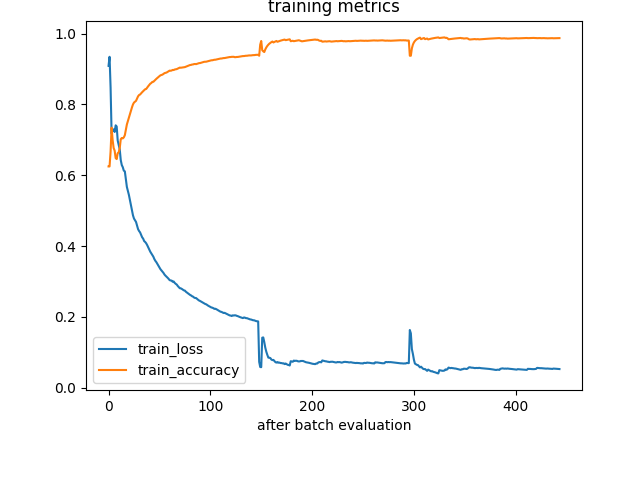
\includegraphics[width=1\linewidth]{training_metrics}
	\caption{Training Loss and Accuracy}
	\label{A subfigure label}
\end{subfigure}%
\begin{subfigure}{.5\textwidth}
	\centering
	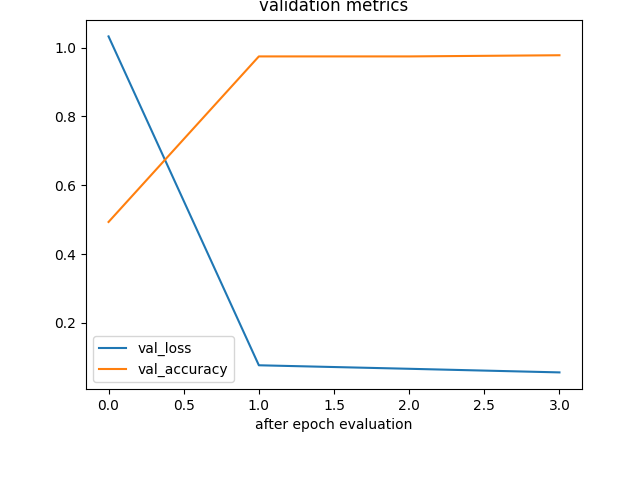
\includegraphics[width=1\linewidth]{validation_metrics}
	\caption{Validation Loss and Accuracy}
	\label{A subfigure label}
\end{subfigure}
\caption{Evaluation metrics observed during training. \textit{Keras} does not provide an interface to register validation metrics after evaluation on one batch, thus the short x-axis. The apparent spikes in the training metrics at the start of every new epoch appear due to the train-set size not being divisible by the batch size into an integer, slightly distorting metric-calculation}
\label{figure label}

\end{figure}
\section{Interpretability: Integrated Gradient}
Once trained, it is difficult to ascertain if the model is picking up on globally salient features as a result of which it assigns correct labels. One visually intuitive technique is the integrated gradient which allows to contrast the activation of each individual pixel between a target-image and one of randomness, called the baseline (black and white are also often used).
It does so by approximating and aggregating the the change per pixel in terms of its gradient over a number of interpolation-steps between the baseline image and the target image.
\newline
Ideally, once the per-pixel activation is visualized, it should resemble certain shapes or patterns that are present in the target image on the basis of which the model has then correctly attributed a correct label. If this isn't the case, despite the label being correct, one might wonder why the model's assigned label was correct and it can be indicative of sensitivity, lack of general interpretability or something else.
\newline
We've applied the integrated gradient to three images on our trained model to investigate if humanly comprehensible features were extracted and are used as a decision-making basis. Below illustrated are three pictures with one of each class, i.e. \textit{interior}, \textit{dish} and \textit{other}. The pictures suggest the model did indeed learn genuine properties of the objects and spaces it is supposed to classify. That is most acutely visible in image (a) where the highlights trace the rim of the plate and its contents. 
\begin{figure}
\centering
\begin{subfigure}{.5\textwidth}
	\centering
	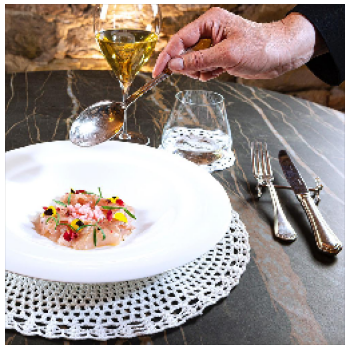
\includegraphics[width=.9\linewidth]{full_295063}
	\caption{Image of class \textit{dish}}
	\label{A subfigure label}
\end{subfigure}%
\begin{subfigure}{.5\textwidth}
	\centering
	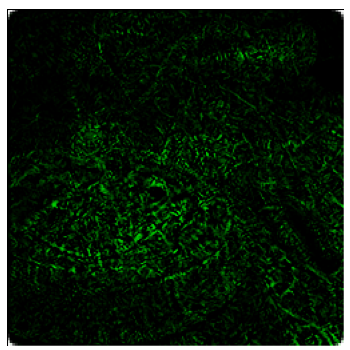
\includegraphics[width=.9\linewidth]{IG_295063}
	\caption{}
	\label{A subfigure label}
\end{subfigure}
\begin{subfigure}{.5\textwidth}
	\centering
	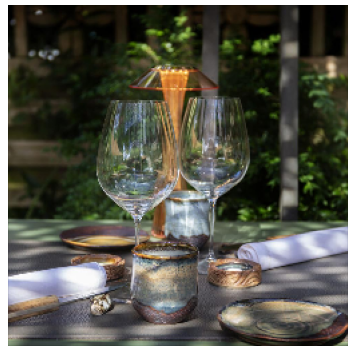
\includegraphics[width=.9\linewidth]{full_glasses}
	\caption{Image of class \textit{interior}}
	\label{A subfigure label}
\end{subfigure}%
\begin{subfigure}{.5\textwidth}
	\centering
	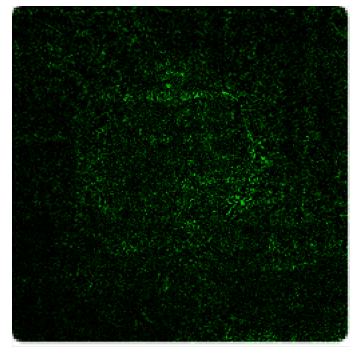
\includegraphics[width=.9\linewidth]{IG_glasses}
	\caption{}
	\label{A subfigure label}
\end{subfigure}
\begin{subfigure}{.5\textwidth}
	\centering
	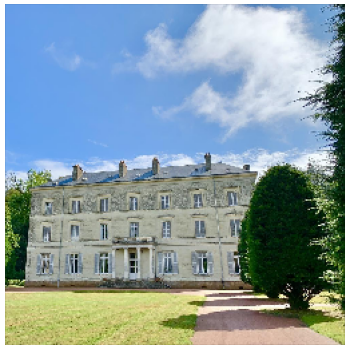
\includegraphics[width=.9\linewidth]{full_243378}
	\caption{Image of class \textit{other}}
	\label{A subfigure label}
\end{subfigure}%
\begin{subfigure}{.5\textwidth}
	\centering
	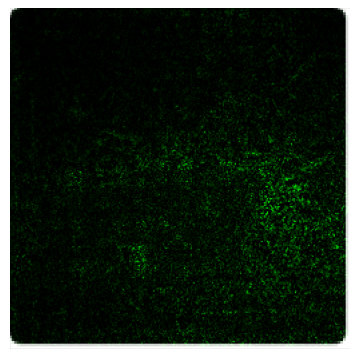
\includegraphics[width=.9\linewidth]{IG_243378}
	\caption{}
	\label{A subfigure label}
\end{subfigure}
\caption{Integrated Gradient}
\label{figure label}
\end{figure}
\newline 
For the interior (c) it is less striking, yet when observing multiple iterations it is clear that the model delineates the wine-glasses. \newline Least convincing is image (e), although windows and the entrance are dimly contrasted along with the tree on the right-hand side and the general square shape of the mansion is crudely captured.
\newline
\newline
This behaviour makes sense, though, as the underlying model is trained on the ImageNet dataset and is thence innately able to recognize objects such as glasses, plates, cutlery which are strongly associated with the first two categories our model is supposed to classify but not with the "lump"-category \textit{other}. Still, given the overall accuracy of 98\% there is no pressing need to fine-tune or further tweak our model as all other categories next to \textit{interior} and \textit{dish}, which seem to come naturally to the pre-trained model, are comprising the \textit{other} category and are consequentially easily separated.
\newline
It is also worth mentioning that, depending on the baseline-image used for the integrated gradient method, the highlighted features are least robust, i.e. most varied, for the class \textit{other} whereas for the other two classes, the visualized integrated gradient is very robust and does not change much when comparing black, white or random noise baseline images. This, once more, reflects the aforementioned point.
\section{Model Application}
The model manages to reliably classify images into the three classes. Figure 3 below displays a set of set of test-images which the model has neither seen in the training-set nor in the validation-set yet has successfully classified. Notice, however, image (i) and image (n) where the prediction is not fully confident. With image (n) the inherent ambivalence of the differentiation between \textit{interior} and \textit{other} might be reflected. Often, certain types of spaces such as gardens or the driveway leading up to a restaurant can not easily be told apart from a place's interior where people dine if, for example, the dining place is within the garden or outdoors. Some ambivalence is introduced as a result.

\begin{figure}
\centering
\begin{subfigure}{.3\textwidth}
	\centering
	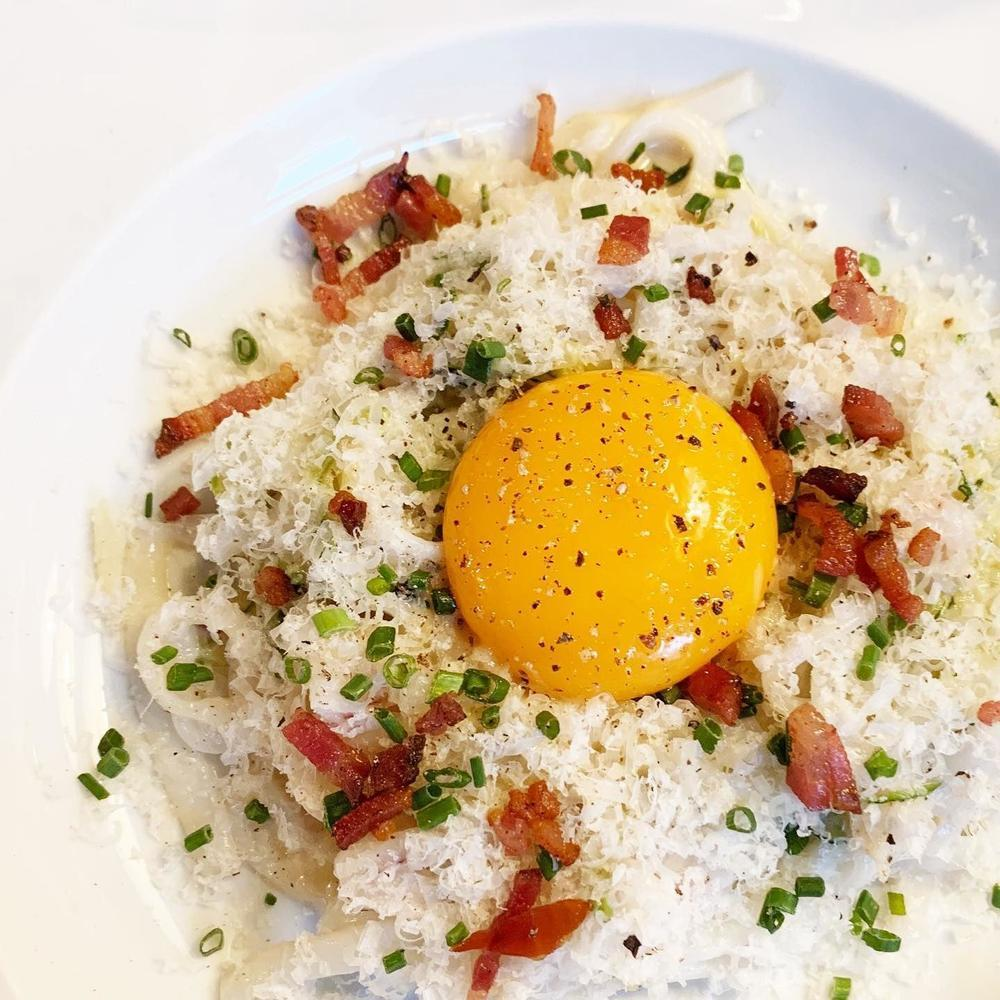
\includegraphics[width=.8\linewidth]{plat1}
	\caption{\textit{dish} 99.9\%}
	\label{A subfigure label}
\end{subfigure}%
\begin{subfigure}{.3\textwidth}
	\centering
	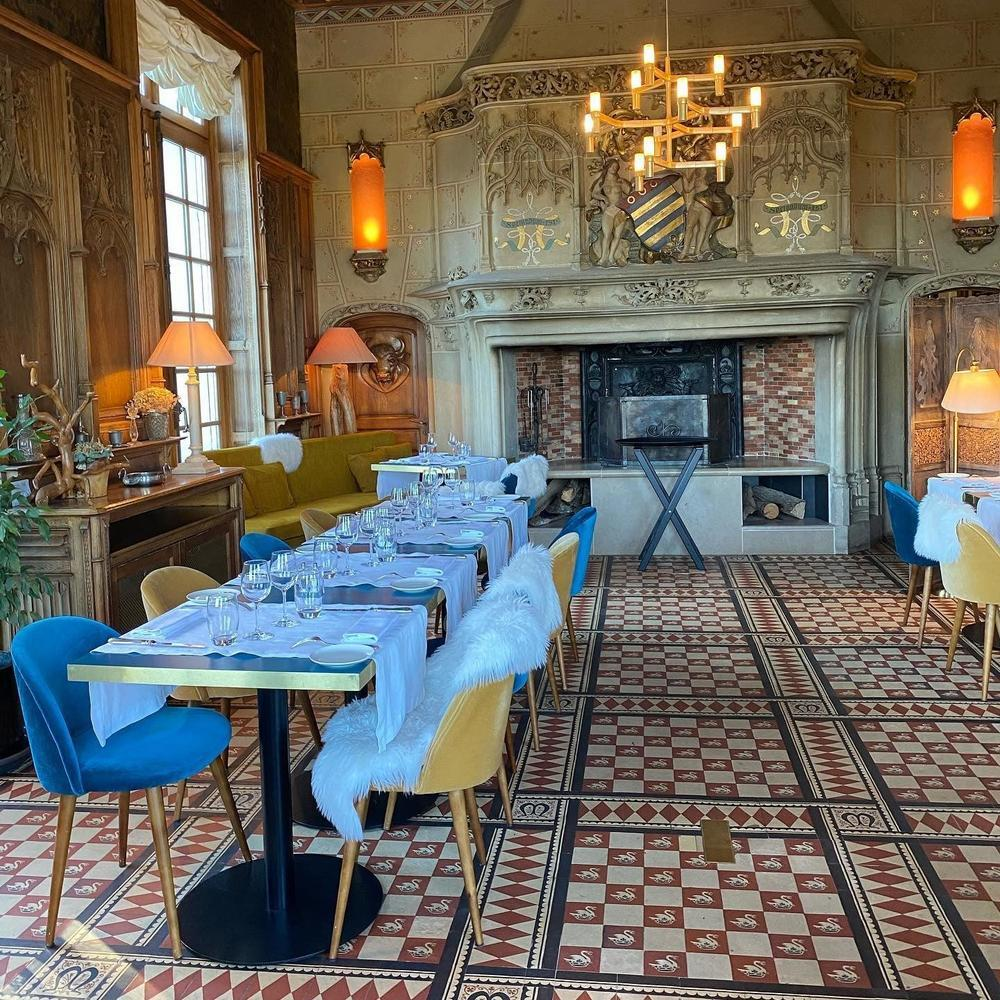
\includegraphics[width=.8\linewidth]{interior1}
	\caption{\textit{interior} 99.2\%}
	\label{A subfigure label}
\end{subfigure}%
\begin{subfigure}{.3\textwidth}
	\centering
	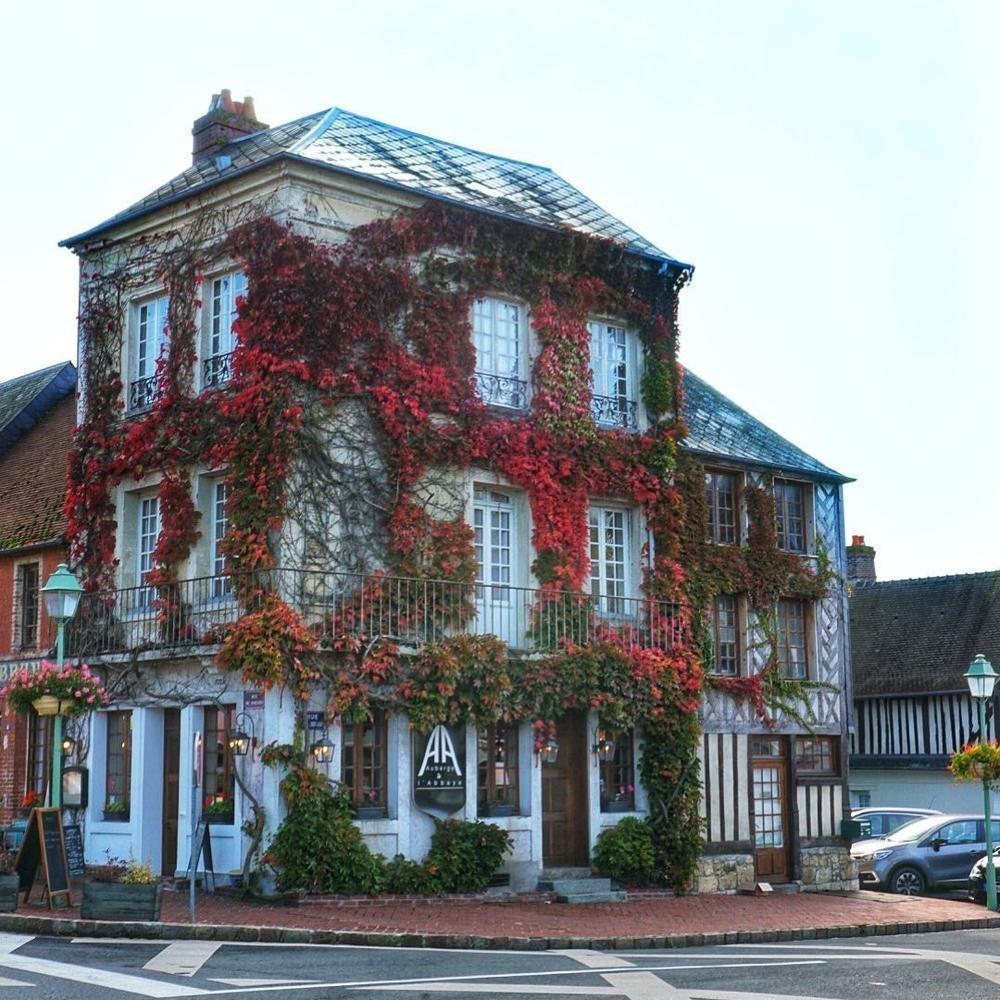
\includegraphics[width=.8\linewidth]{other1}
	\caption{\textit{other} 99.4\%}
	\label{A subfigure label}
\end{subfigure}

\begin{subfigure}{.3\textwidth}
	\centering
	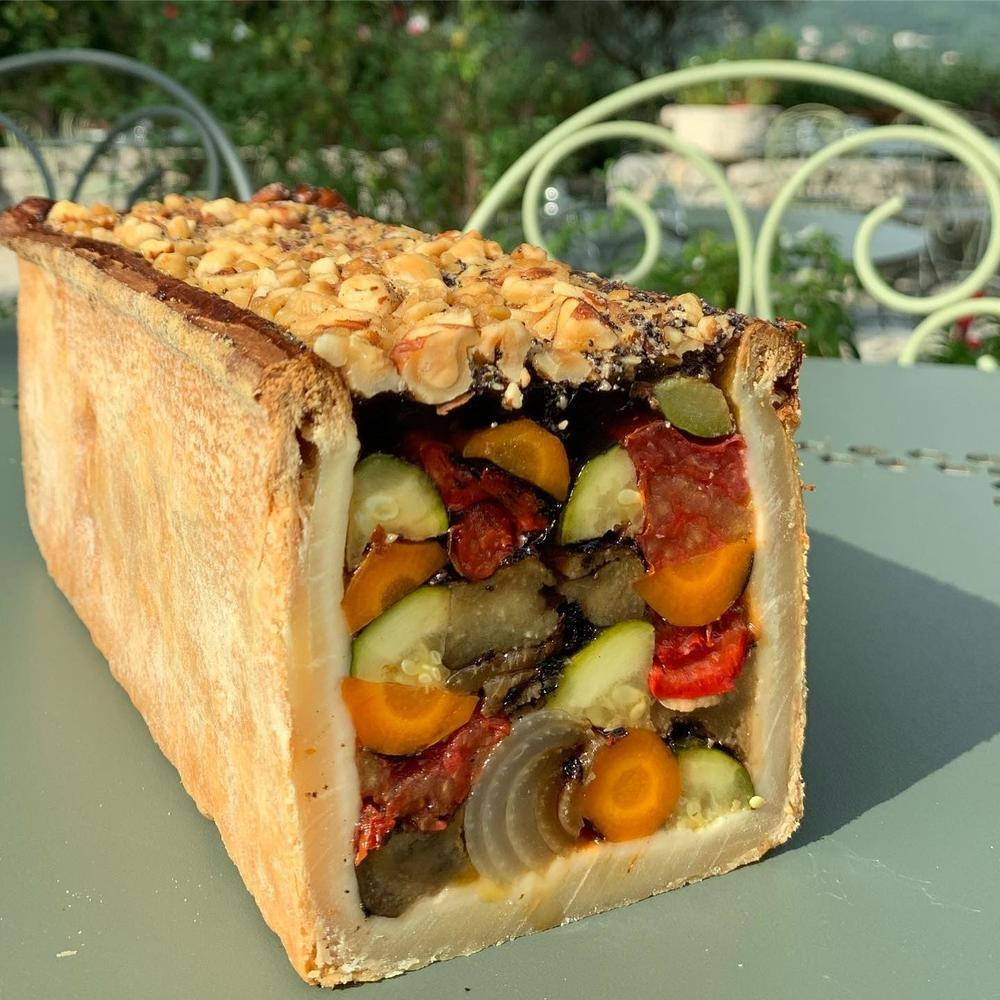
\includegraphics[width=.8\linewidth]{plat2}
	\caption{\textit{dish} 99.9\%}
	\label{A subfigure label}
\end{subfigure}%
\begin{subfigure}{.3\textwidth}
	\centering
	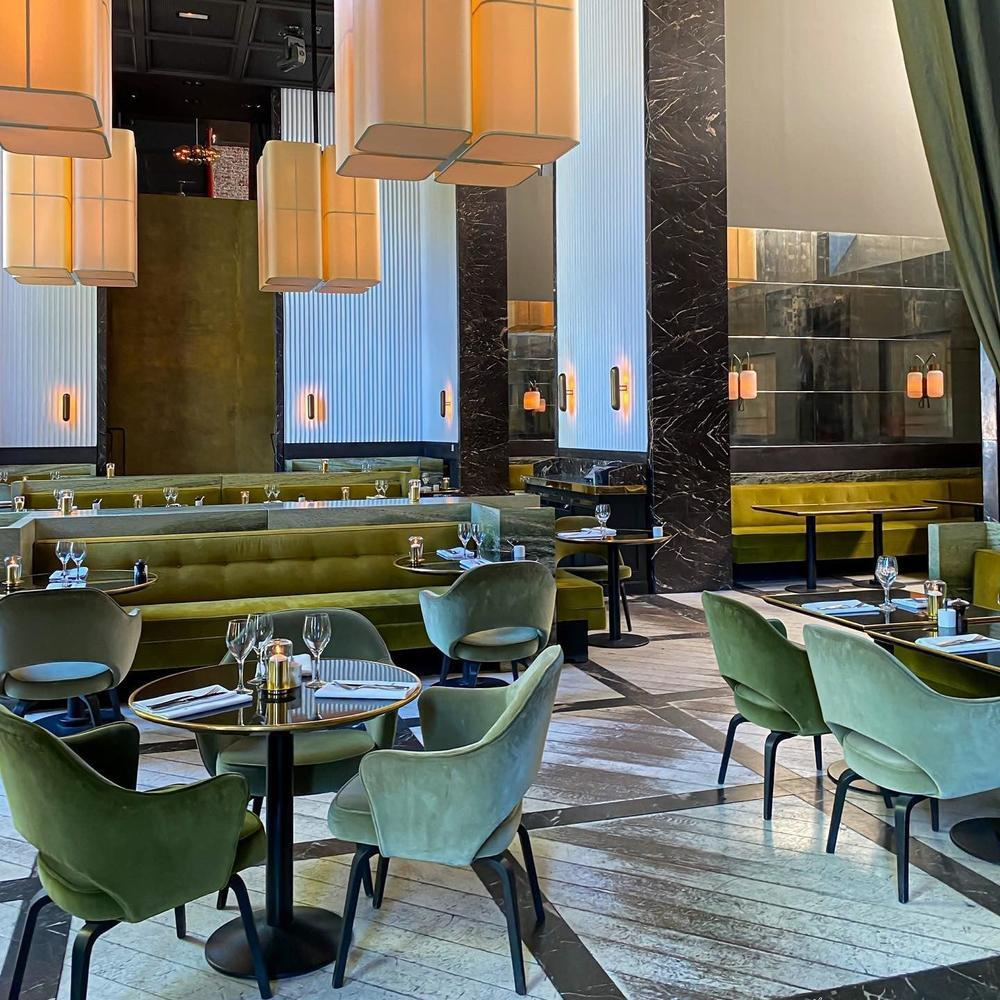
\includegraphics[width=.8\linewidth]{interior2}
	\caption{\textit{interior} 99.3\%}
	\label{A subfigure label}
\end{subfigure}%
\begin{subfigure}{.3\textwidth}
	\centering
	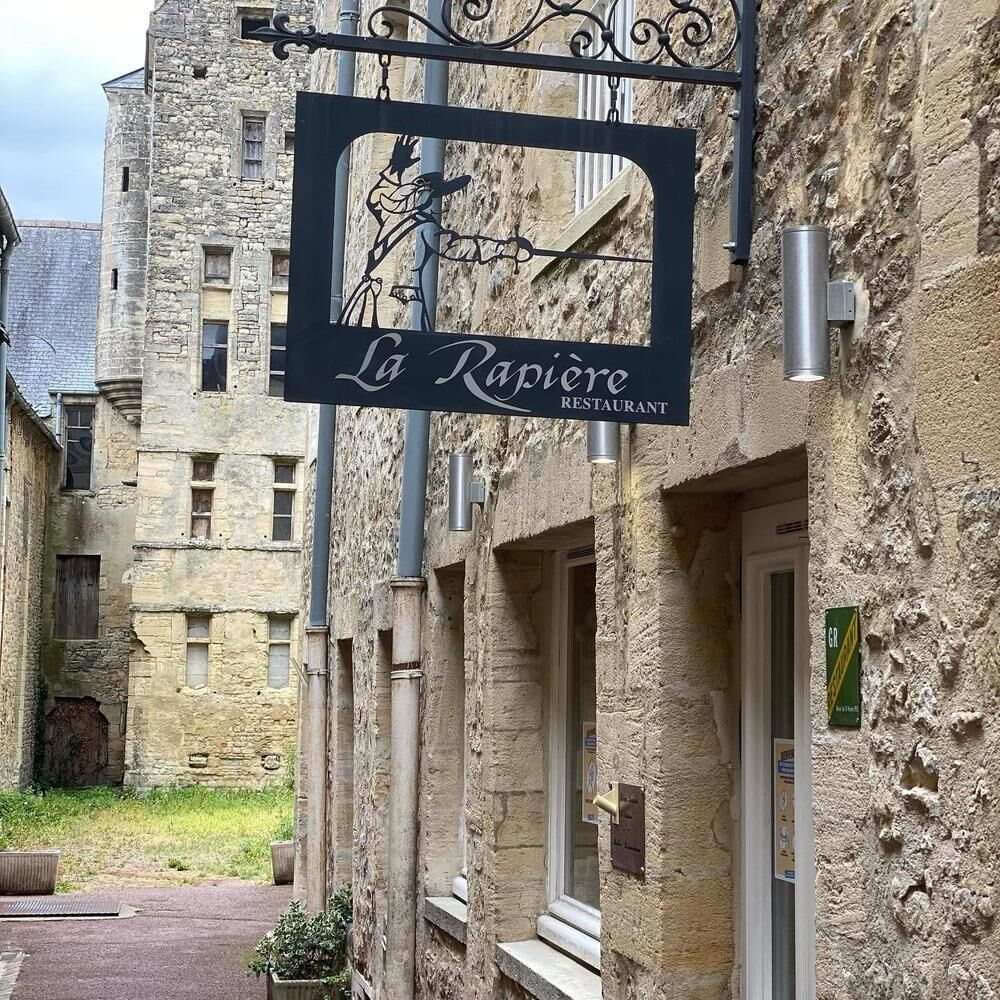
\includegraphics[width=.8\linewidth]{other2}
	\caption{\textit{other} 99.5\%}
	\label{A subfigure label}
\end{subfigure}

\begin{subfigure}{.3\textwidth}
	\centering
	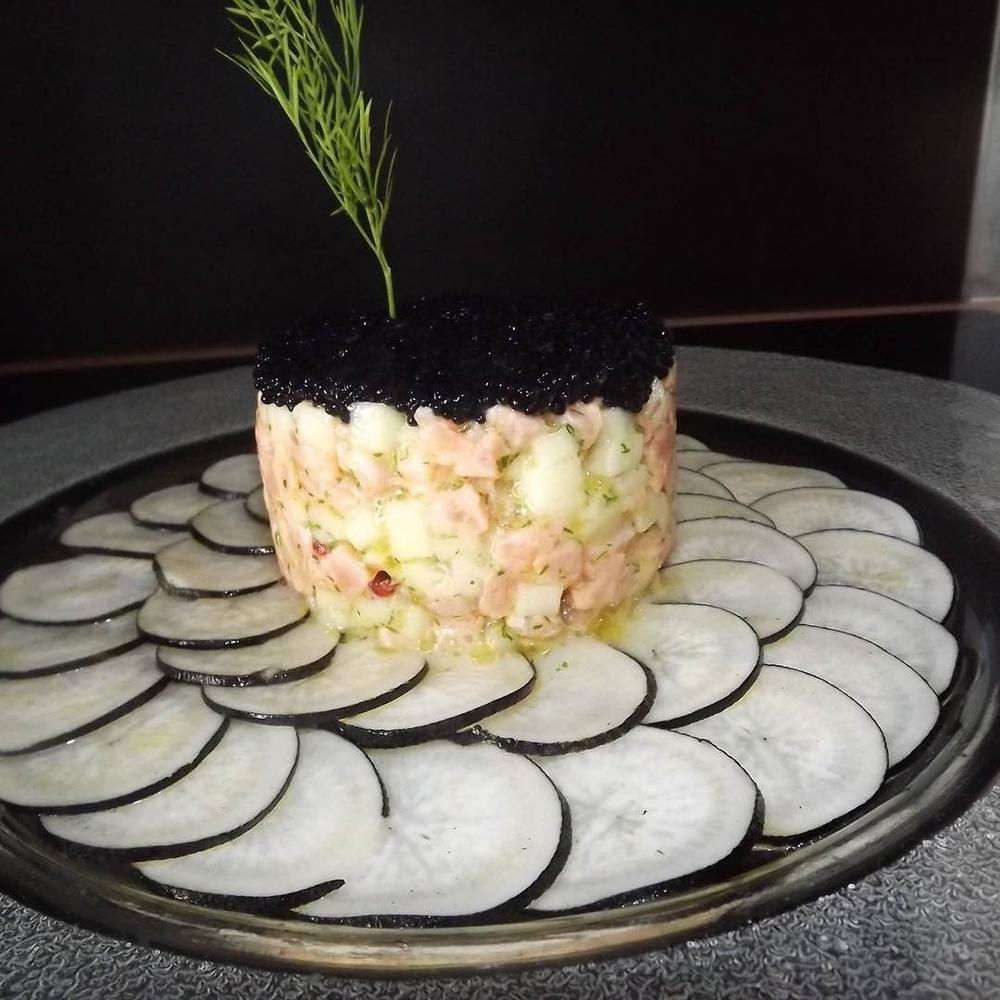
\includegraphics[width=.8\linewidth]{plat3}
	\caption{\textit{dish} 99.4\%}
	\label{A subfigure label}
\end{subfigure}%
\begin{subfigure}{.3\textwidth}
	\centering
	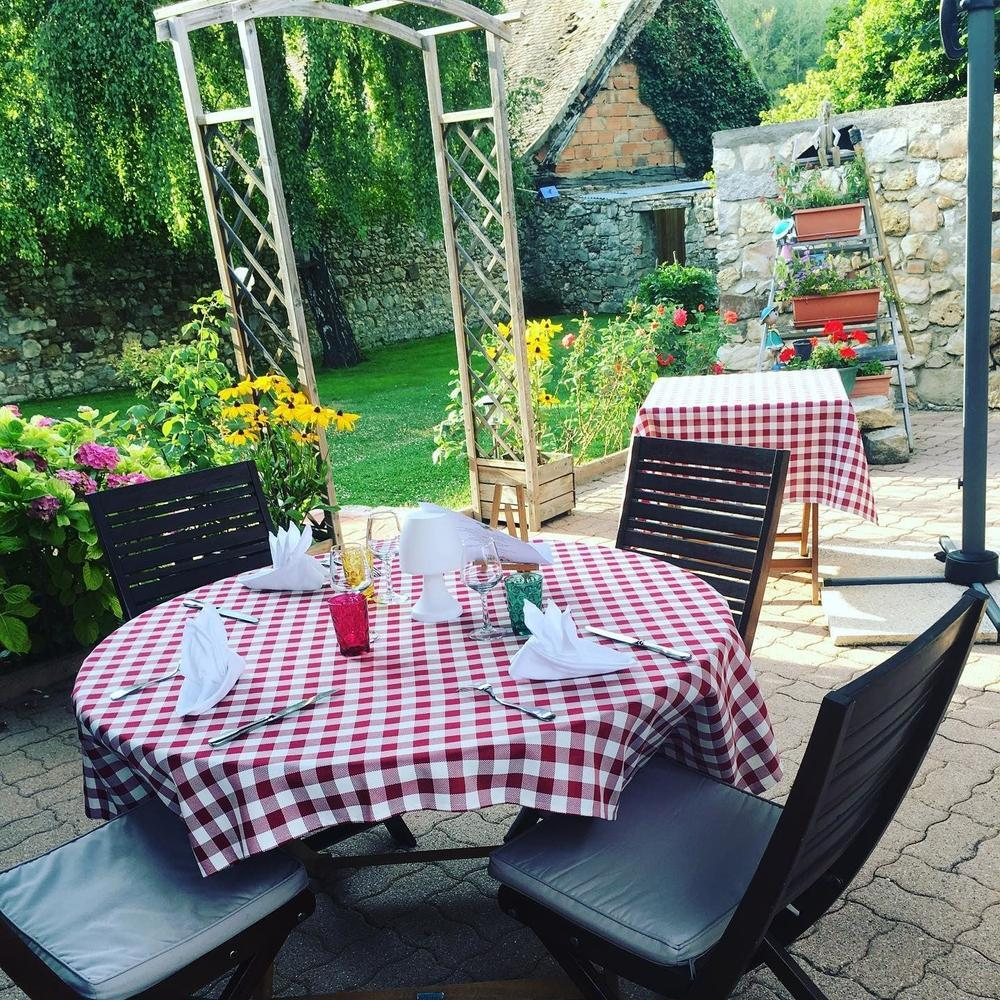
\includegraphics[width=.8\linewidth]{interior3}
	\caption{\textit{interior} 99.3\%}
	\label{A subfigure label}
\end{subfigure}%
\begin{subfigure}{.3\textwidth}
	\centering
	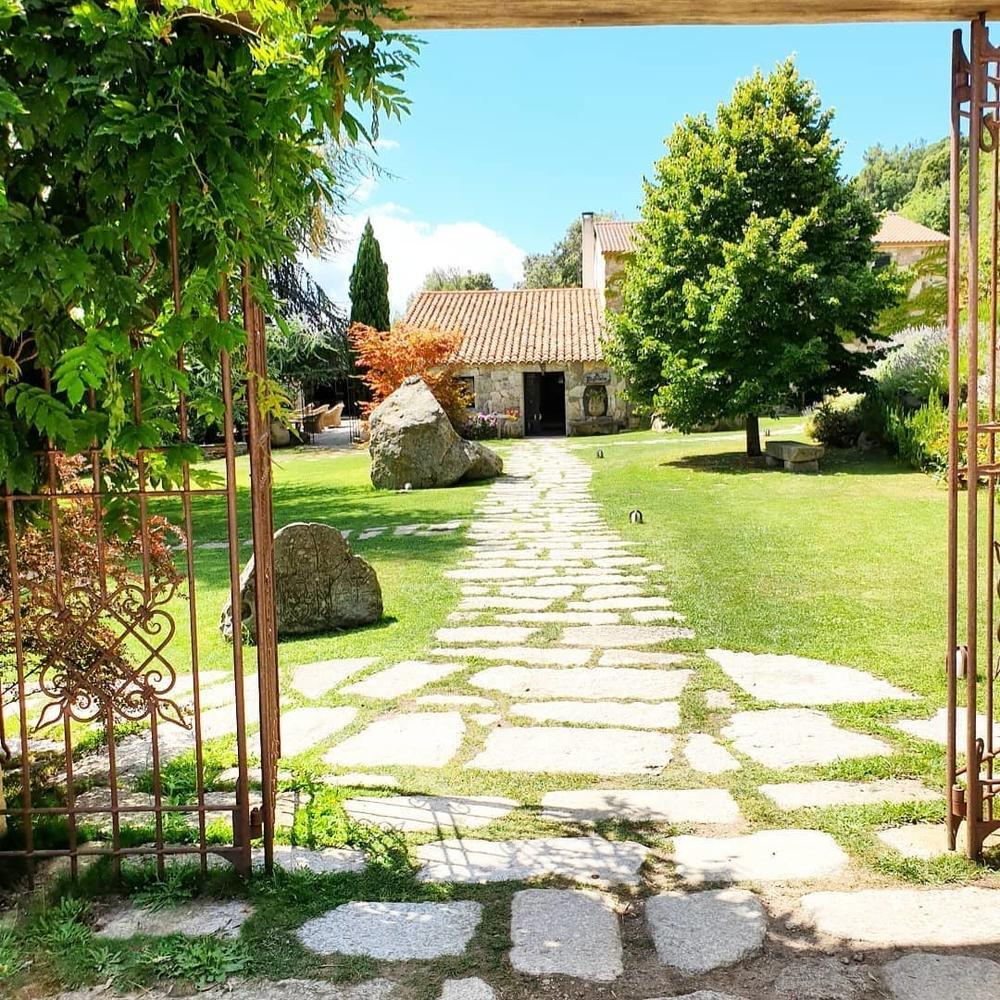
\includegraphics[width=.8\linewidth]{other3}
	\caption{\textit{other} 55.2\%; interior 46\%}
	\label{A subfigure label}
\end{subfigure}

\begin{subfigure}{.3\textwidth}
	\centering
	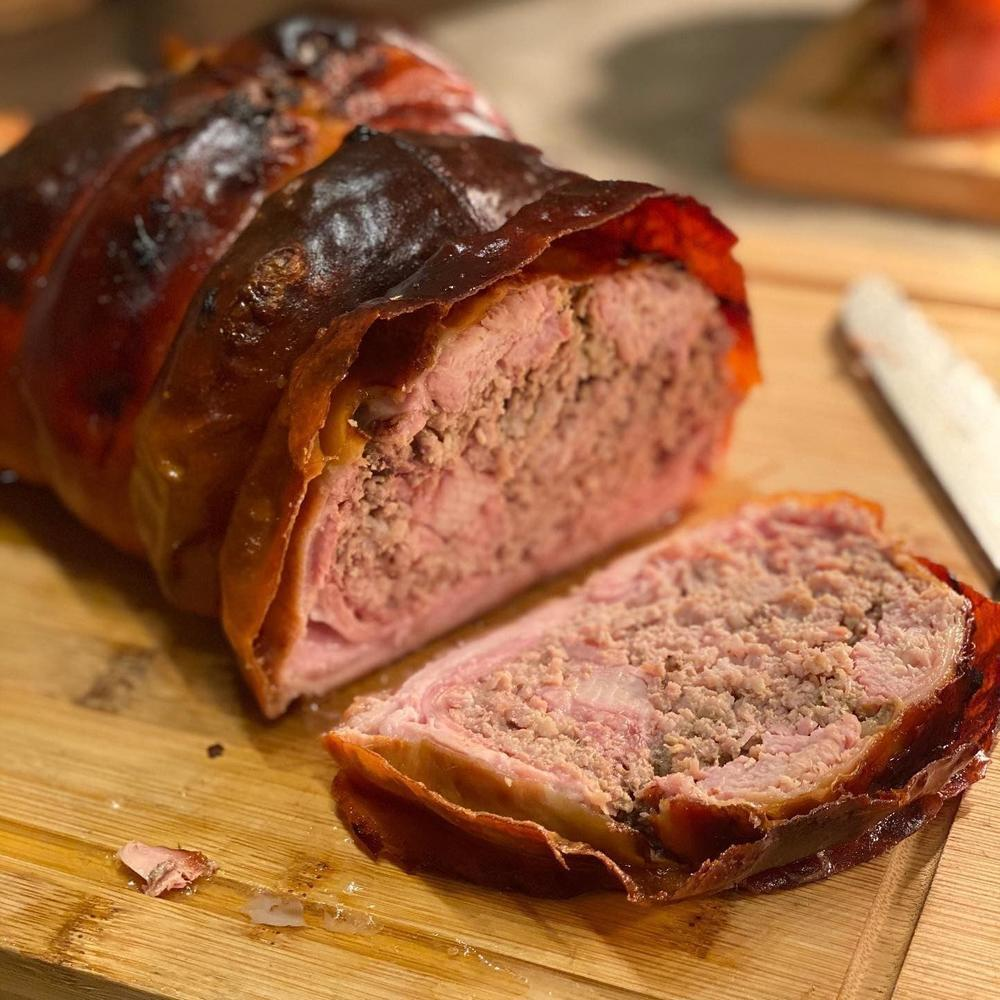
\includegraphics[width=.8\linewidth]{plat4}
	\caption{\textit{dish} 98.0\%}
	\label{A subfigure label}
\end{subfigure}%
\begin{subfigure}{.3\textwidth}
	\centering
	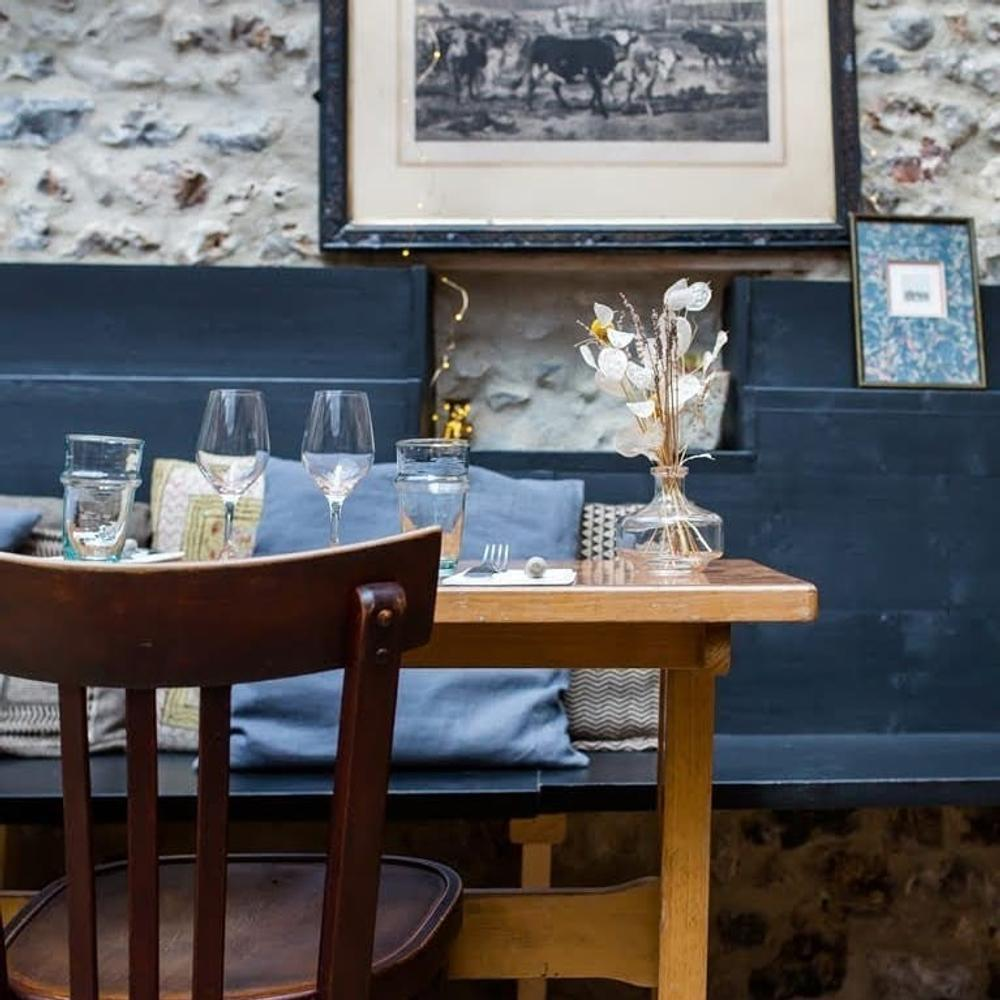
\includegraphics[width=.8\linewidth]{interior4}
	\caption{\textit{interior} 99.8\%}
	\label{A subfigure label}
\end{subfigure}%
\begin{subfigure}{.3\textwidth}
	\centering
	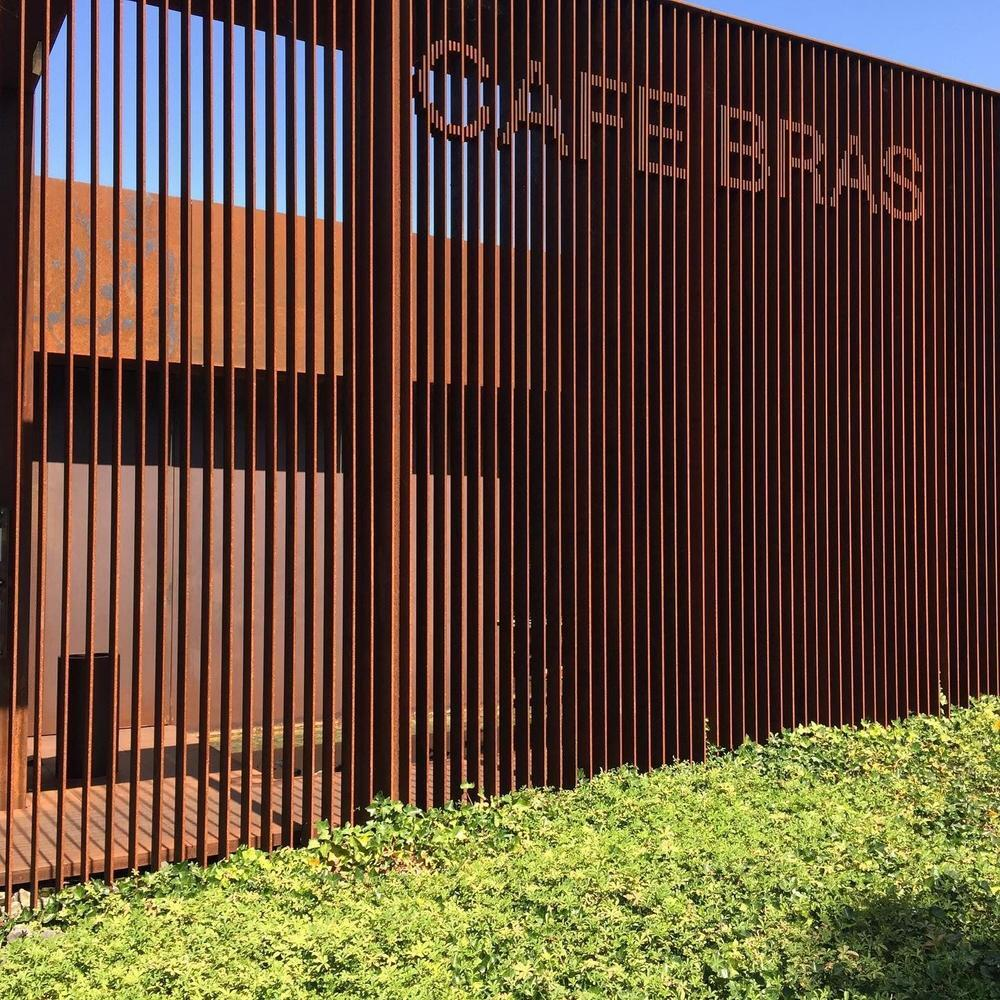
\includegraphics[width=.8\linewidth]{other4}
	\caption{\textit{other} 93.1\%}
	\label{A subfigure label}
\end{subfigure}

\begin{subfigure}{.3\textwidth}
	\centering
	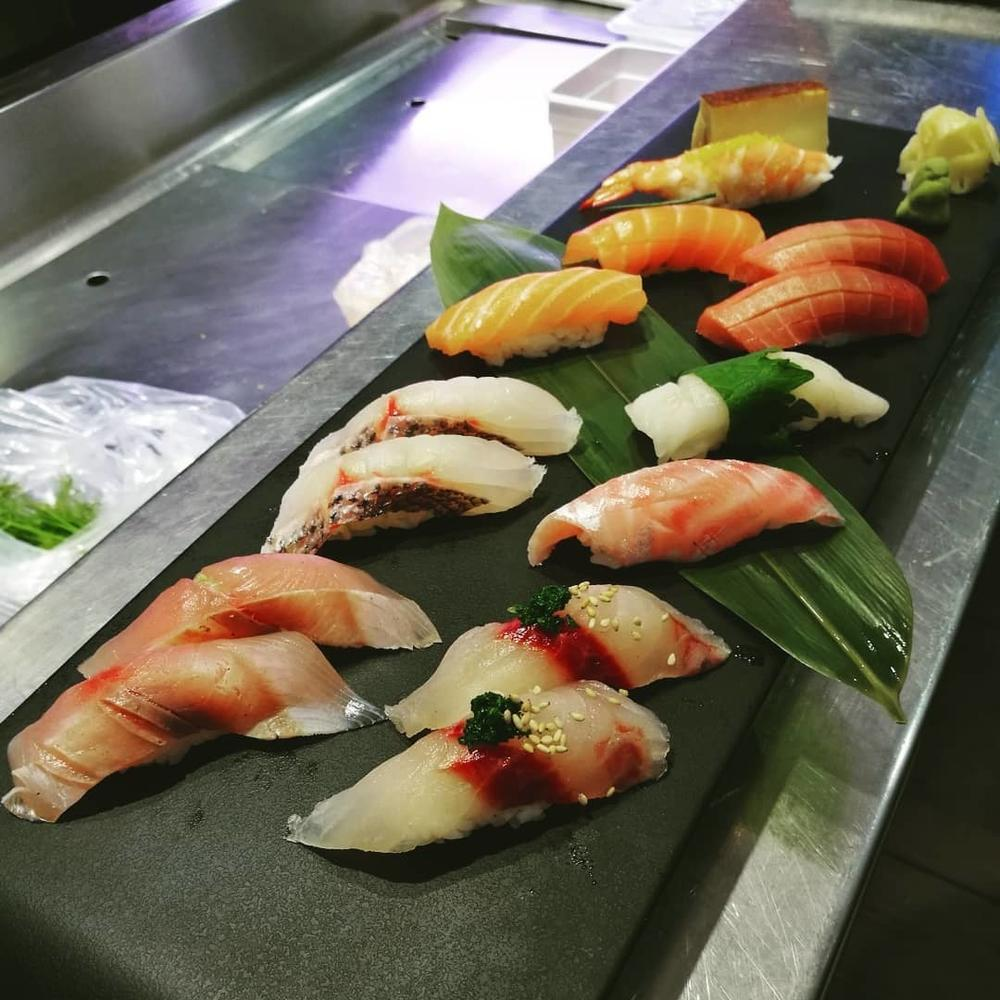
\includegraphics[width=.8\linewidth]{plat5}
	\caption{\textit{dish} 99.9\%}
	\label{A subfigure label}
\end{subfigure}%
\begin{subfigure}{.3\textwidth}
	\centering
	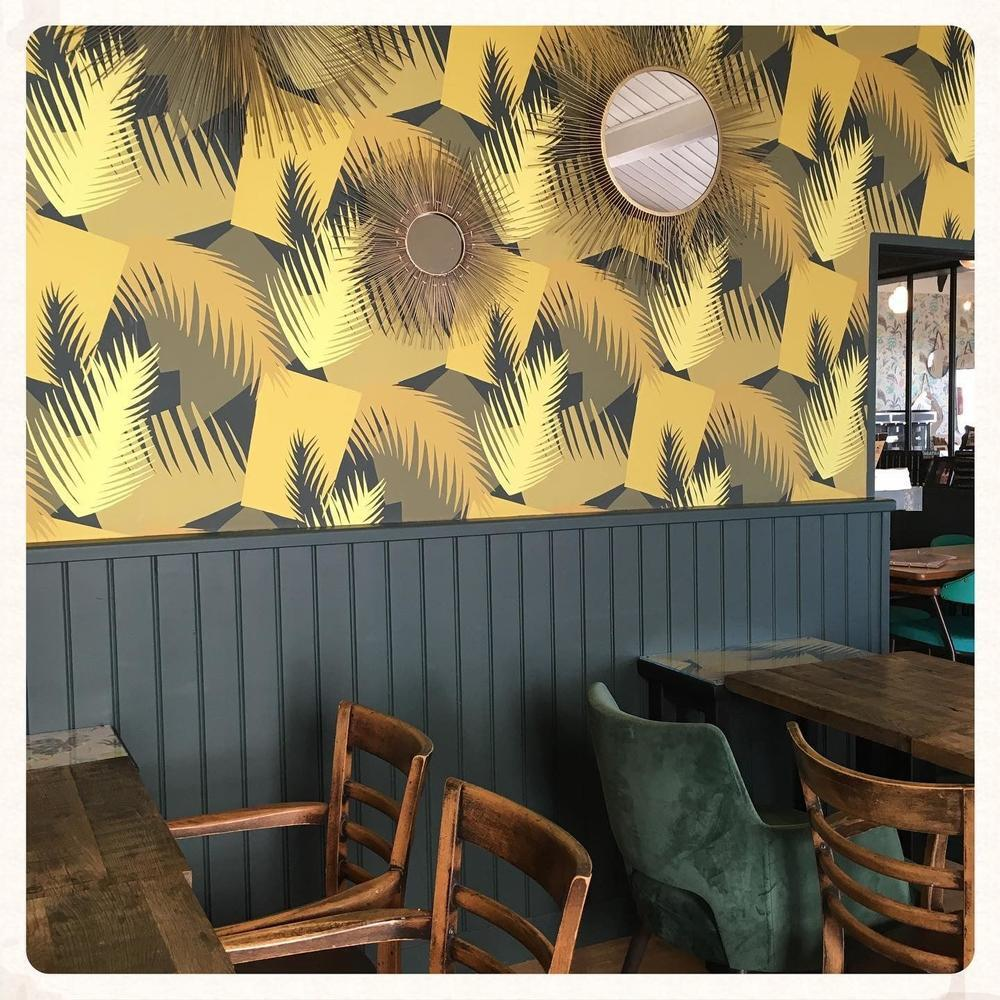
\includegraphics[width=.8\linewidth]{interior5}
	\caption{\textit{interior} 77.5\%; other 21\%}
	\label{A subfigure label}
\end{subfigure}%
\begin{subfigure}{.3\textwidth}
	\centering
	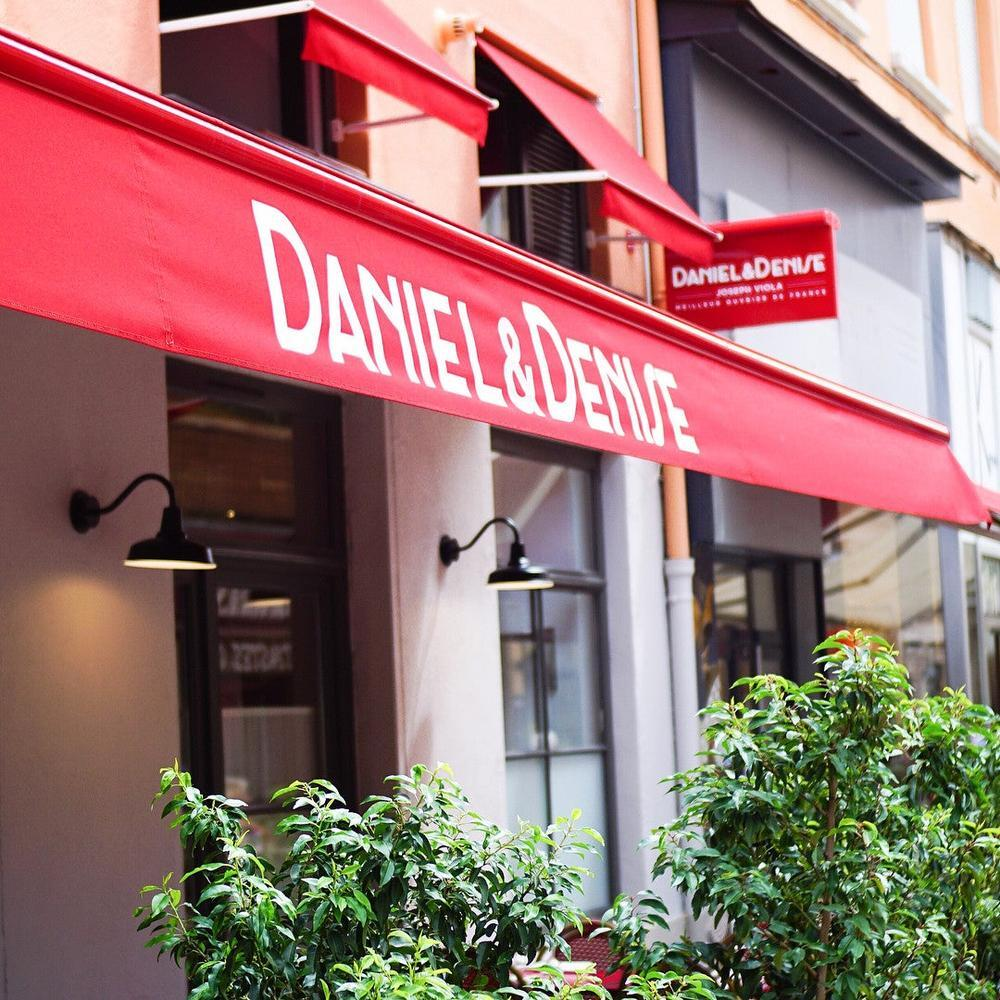
\includegraphics[width=.8\linewidth]{other5}
	\caption{\textit{other} 96.8\%}
	\label{A subfigure label}
\end{subfigure}

\caption{Model predictions on unseen images (class, probability)}
\label{figure label}
\end{figure}

\end{document}  
